\documentclass[xcolor=table, aspectratio=169, usepdftitle=false]{beamer}

\makeatletter
\appto\input@path{{pkgs/awesome-beamer}, {pkgs/smile}}
\makeatother

\usepackage[english, secslide, subsecslide, coloraccent=red]{beamerthemeawesome}

\addbibresource{references.bib}

\usepackage{scrextend}
\usepackage{emoji}
\usepackage{listings}
\usepackage[verbatim=true]{lstfiracode}
\usepackage[hidenotes]{pdfpc}
\usepackage{tikzlings-owls}

\title{In-Memory Processing}
\author{Lukas Pietzschmann}
\subtitle{Am Beispiel von Apache Spark}
\email{lukas.pietzschmann@uni-ulm.de}
\institute{Institut für Verteilte Systeme}
\uni{Universität Ulm}
\location{Ulm}
\date{12. Januar 2023}
\background{pics/sparks.png}

\lstdefinestyle{animateblocks}{
	basicstyle=\ttfamily\color{black!20},
	moredelim=**[is][\only<+>{\color{black}}]{@}{@},
}
\lstset{
	style=FiraCodeStyle,
	basicstyle=\ttfamily,
	commentstyle=\color{gray}\itshape,
	keywordstyle=\bfseries,
	escapeinside={<!}{!>},
}

\lstdefinelanguage{Python}{
	morekeywords={access, and, break, class, continue, def, del, elif, else,%
		except, exec, finally, for, from, global, if, import, in, is, lambda,%
		not, or, pass, print, raise, return, try, while},
	morekeywords=[2]{range},
	sensitive=true,
	morestring=[b]',
	morestring=[b]",
	morecomment=[s]{'''}{'''},
	morecomment=[l]{//},
	morecomment=[s]{"""}{"""},
	morestring=[s]{r'}{'},
	morestring=[s]{r"}{"},
	morestring=[s]{r'''}{'''},
	morestring=[s]{r"""}{"""},
	morestring=[s]{u'}{'},
	morestring=[s]{u"}{"},
	morestring=[s]{u'''}{'''},
	morestring=[s]{u"""}{"""}
}

\begin{document}

\maketitle

% \input{slides/agenda.tex}
\section{Intro}
\begin{frame}{Motivation}
	\begin{columns}[T]
		\begin{column}{0.45\textwidth}
			Festplatten-Geschwindigkeit:
			
\includegraphics[width=0.75\textwidth]{pics/slow.jpg}\\
			\tiny\url{https://i.redd.it/1qh4lphop3501.jpg}
		\end{column}
		\begin{column}{0.45\textwidth}
			RAM-Geschwindigkeit:
			
\includegraphics[width=0.9\textwidth]{pics/speed.jpg}\\
			\tiny\url{https://i.kym-cdn.com/entries/icons/original/000/028/987/lightningspeed.jpg}
		\end{column}%
	\end{columns}
	\pause
	\vspace{1em}
	$\Rightarrow$~Auswertung in Echtzeit, unabhängig der Datenmenge
\end{frame}

\begin{frame}{Motivation}
	\only<1>{
		\begin{table}[]
		\begin{tabular}{r|cc}
			\hline
									& \textbf{Split sizes (MB)} & \textbf{Execution time (s)} \\
			\hline\hline
			MapReduce input splits  & 128                       & 2376                        \\
			Spark input splits      & 256                       & 1392                        \\
			MapReduce shuffle       & 100                       & 2371                        \\
			Spark shuffle           & 300                       & 1334                        \\ \hline
		\end{tabular}
		\caption{Best execution time of MapReduce and Spark with WordCount workload~\cite[12]{ahmed2020comprehensive}}
		\end{table}
	}

	\only<2>{
		\begin{table}[]
		\begin{tabular}{r|cc}
			\hline
									& \textbf{Split sizes (MB)} & \textbf{Execution time (s)} \\
			\hline\hline
			MapReduce input splits  & 256                       & 21014                       \\
			Spark input splits      & 512                       & 3780                        \\
			MapReduce shuffle       & 150                       & 24250                       \\
			Spark shuffle           & 128                       & 6540                        \\ \hline
		\end{tabular}
		\caption{Best execution time of MapReduce and Spark with Terasort workload~\cite[14]{ahmed2020comprehensive}}
		\end{table}
	}
	\only<3>{
		\begin{figure}
			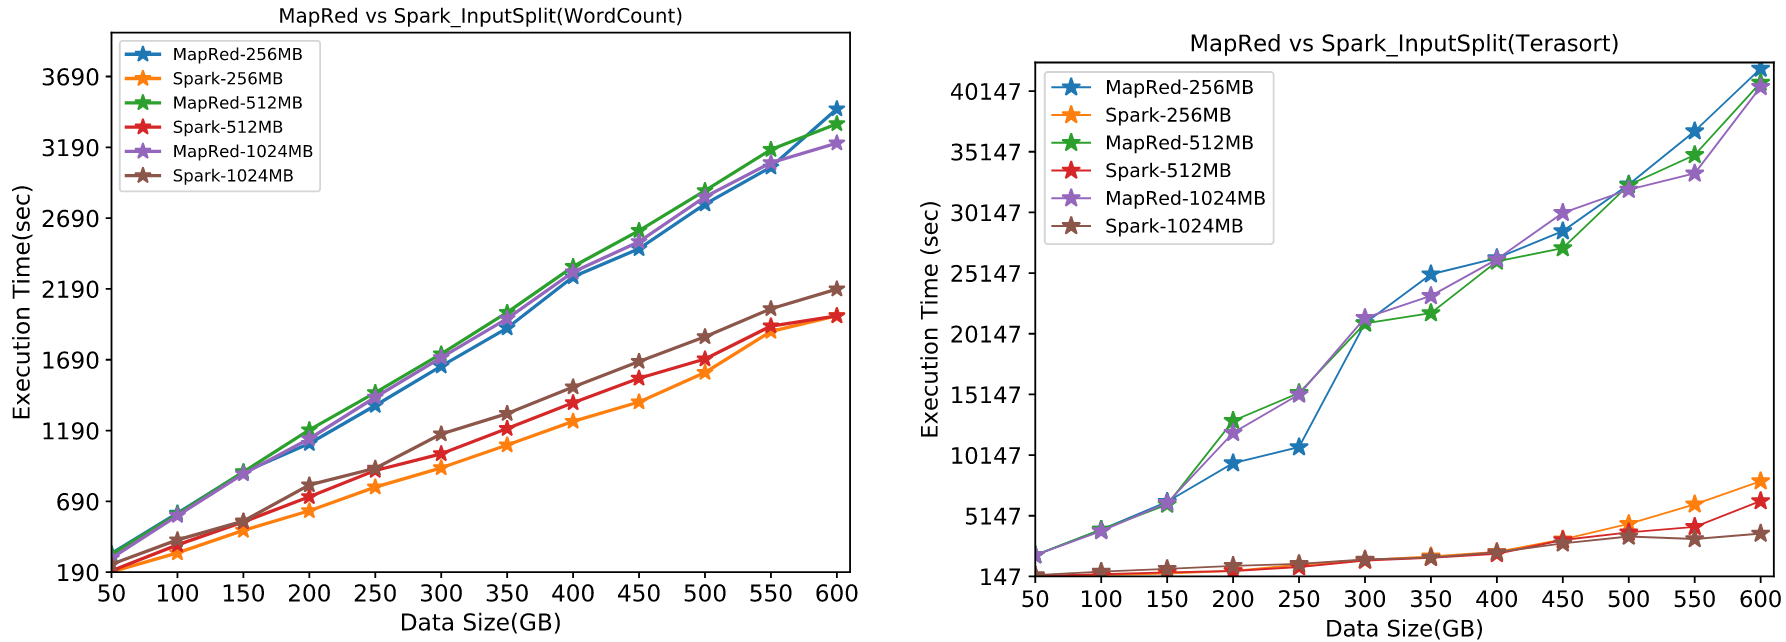
\includegraphics[width=\textwidth]{pics/MapRedvsSpark.png}
			\caption{Comparison of Hadoop and Spark with WordCount and TeraSort workload with varied input splits and shuffle tasks~\cite[14]{ahmed2020comprehensive}}
		\end{figure}
	}
\end{frame}

% \begin{frame}{Mögliche Fragen}
% 	\begin{itemize}
% 		\item Was passiert wenn der komplette Adressraum belegt ist?
% 		\item Wie können bereits erzeugte Daten geschützt werden?
% 		\item Betreibt nicht jeder Computer In-Memory Processing?
% 	\end{itemize}
% \end{frame}

\section{Lernziele}
\begin{frame}{Lernziele}{Theorie}
	\begin{itemize}
		\item Unterschied zwischen reinem Map-Reduce und Spark erkennen
		\item Sparks Datenmodell und dessen Implikationen verstehen
		\item Wichtige Bindeglieder und deren Rolle vom Programmieren bis zur Ausführung kennen
		\item Zumindest von der Existenz weiterer Spark-Bibliotheken wissen
	\end{itemize}
\end{frame}

\begin{frame}{Lernziele}{Praxis}
	\begin{columns}
		\begin{column}{0.7\textwidth}
			\begin{itemize}
				\item Verschiedene Aktionen und Transformationen
				\begin{itemize}
					\item kennen,
					\item anwenden und
					\item kombinieren
				\end{itemize}
					können (und das natürlich sinnvoll)
				\item<2> Wörter-zählen in Spark implementieren können \emoji{wink}
			\end{itemize}
		\end{column}
		\begin{column}{0.2\textwidth}
			\only<2>{
				\begin{tikzpicture}[
					remember picture,
					overlay,
				]
					\owl[yshift=-1.5cm, xshift=1cm, magichat, speech={1,2,3,...}]
				\end{tikzpicture}
			}
		\end{column}
	\end{columns}
\end{frame}
\section{In-Memory Processing}
\begin{frame}{Übersicht}
	\begin{columns}[T]
		\begin{column}{0.45\textwidth}
			\textbf{Anwendungsfälle}
			\pdfpcnote{- Realtime vs Near-Realtime}
			\pdfpcnote{- Realtime: Selbstfahrende Autos}
			\pdfpcnote{- Neartime: Daten zeitnah vorhanden (Sektunden, Minuten, Stunden). System Monitoring}
			\begin{itemize}
				\item Echtzeit-Systeme
				\begin{itemize}
					\item Zahlungsverarbeitung
					\item Börsenhandel
					\item Simulationen
					\item BI
					\item ...
				\end{itemize}
			\end{itemize}
		\end{column}
		\begin{column}{0.45\textwidth}
			\textbf{Implementierungen}
			\begin{itemize}
				\item SAP Hana
				\item Apache Flink
				\pause
				\item \emoji{sparkles}Apache Spark\emoji{sparkles}
			\end{itemize}
		\end{column}
	\end{columns}
\end{frame}
\section{Apache Spark}

\subsection{Übersicht}
\begin{frame}{Historie}
	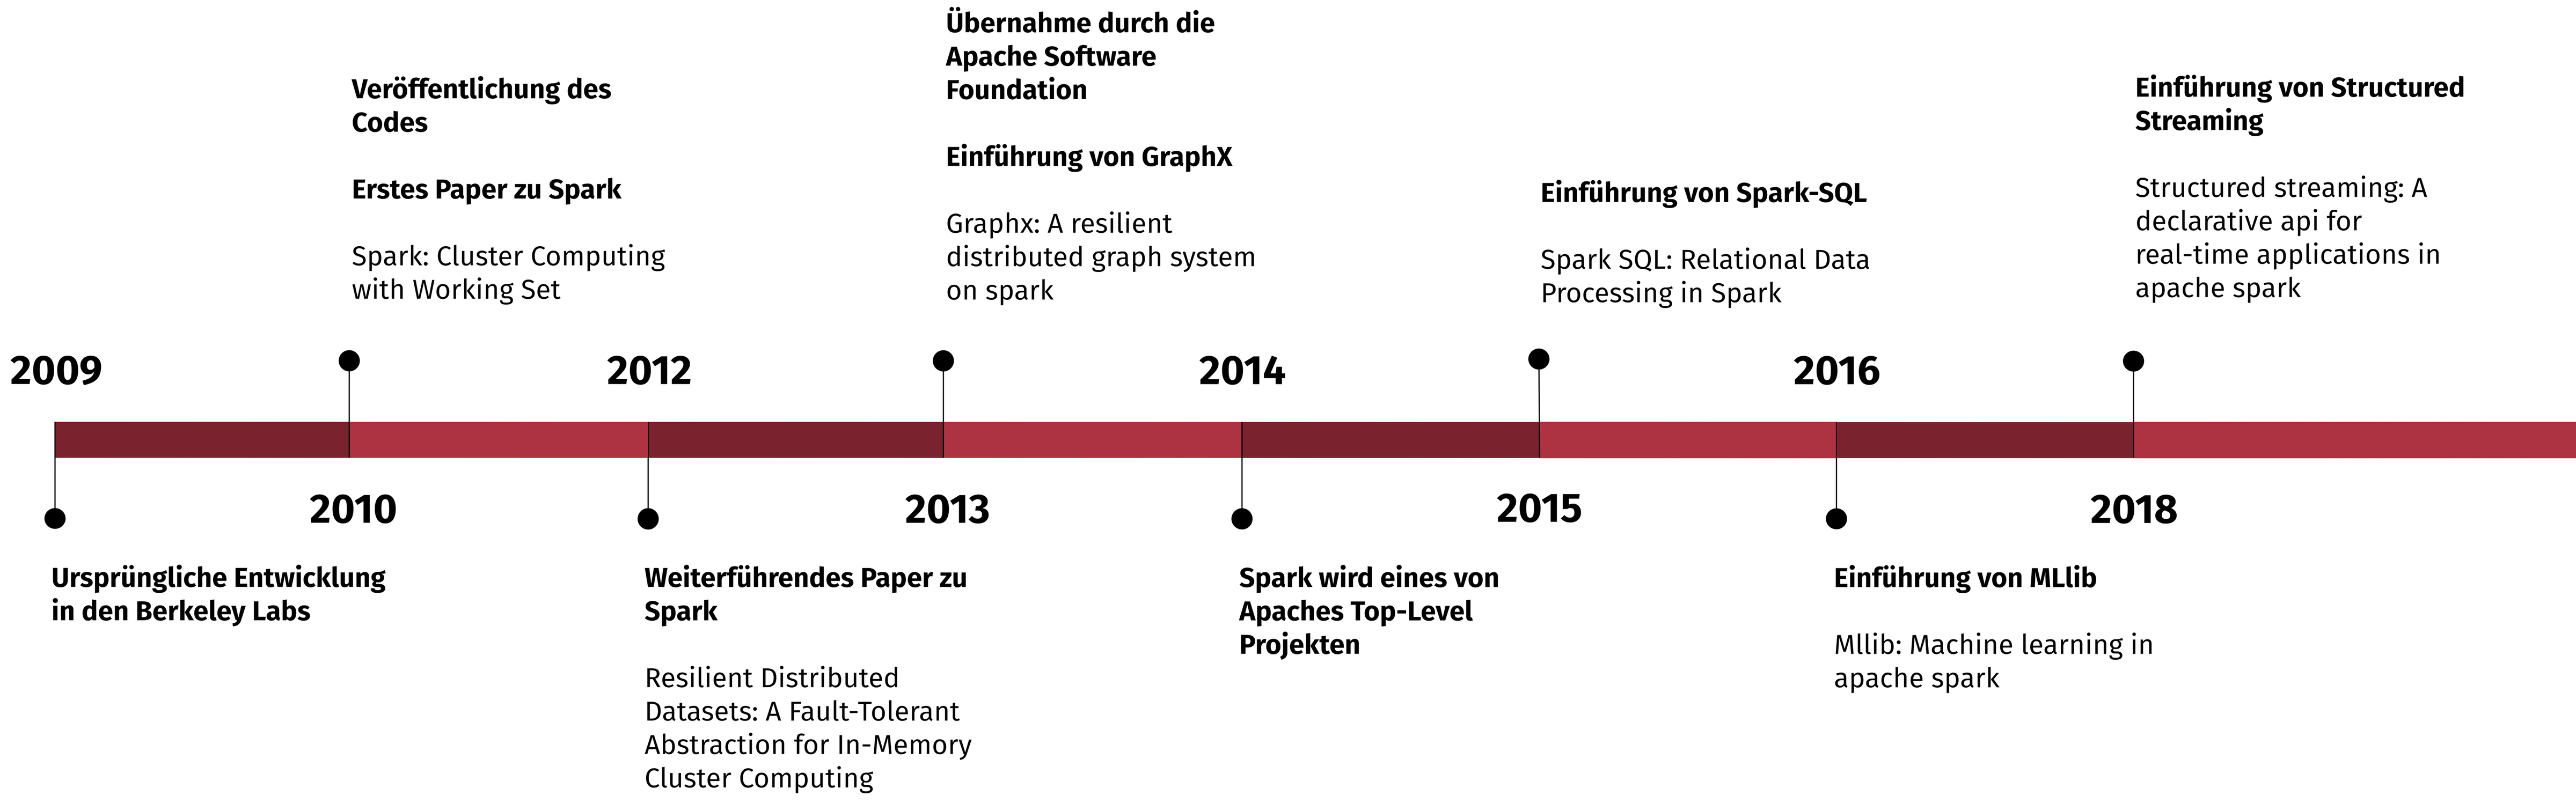
\includegraphics[width=1.1\textwidth]{pics/Papers.png}
\end{frame}
% https://stanford.edu/~rezab/sparkclass/slides/itas_workshop.pdf Seite 46

\begin{frame}{Ziele}
	\enquote{\textcolor{gray}{
		[...] \textcolor{accent}{reuse} a working set of
		\textcolor{accent}{data across multiple parallel operations}. This includes many
		\textcolor{accent}{iterative machine learning algorithms}, as well as
		\textcolor{accent}{interactive data analysis} tools. We propose a new framework
		called Spark that supports these applications while \textcolor{accent}{retaining}
		the \textcolor{accent}{scalability} and \textcolor{accent}{fault tolerance} of MapReduce.
	}}~~\cite[1]{zaharia2010spark}
	\\
	\uncover<2->{+ mehr Möglichkeiten als reines Map-Reduce}
	% 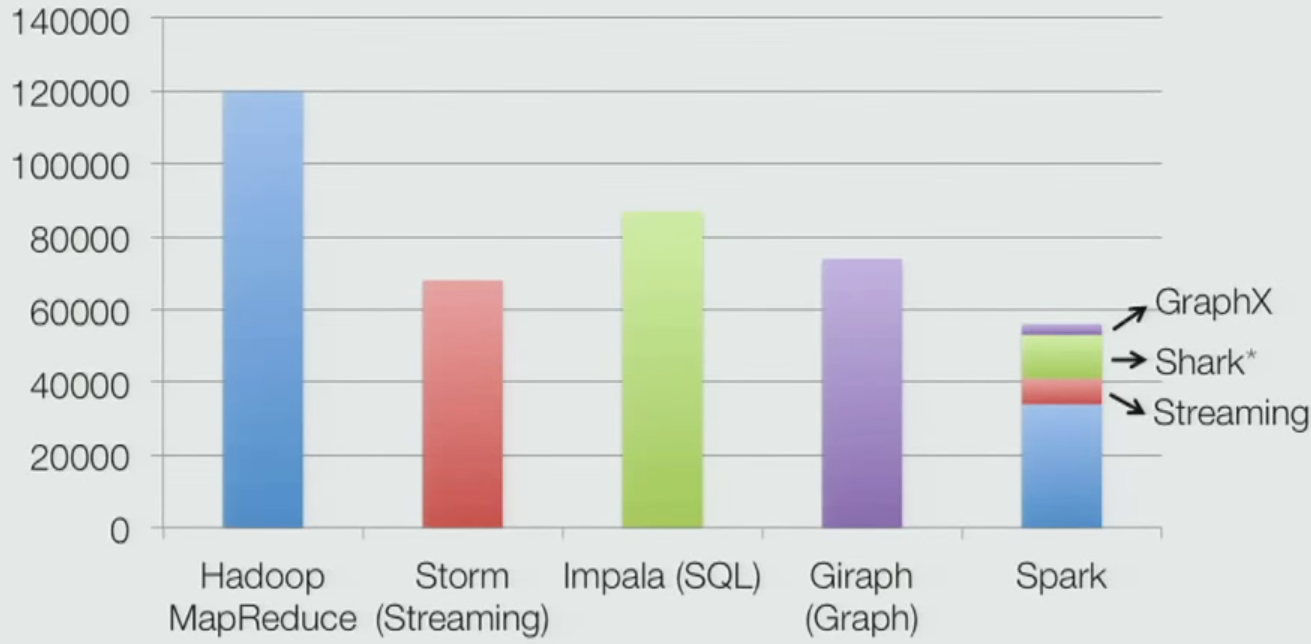
\includegraphics[width=0.75\textwidth]{pics/CodeSize.png}\\
	% \tiny\url{https://youtu.be/nU6vO2EJAb4?t=1585}
\end{frame}

\begin{frame}{Übersicht}
	\begin{itemize}
		\item Generalisiertes Map-Reduce\\\Rightarrow~Größere Bandbreite an Anwendungsfällen
		\item Interaktive Shell + Java-API
		\begin{itemize}
			\item Python (\texttt{pyspark})
			\item Scala (\texttt{spark-shell})
			\item R (\texttt{sparkR})
		\end{itemize}
		\item Ausführung auf
		\begin{itemize}
			\item Einzelnen Maschinen
			\item Clustern aus mehreren Maschinen
		\end{itemize}
	\end{itemize}
\end{frame}

\subsection{Datenmodell}
\begin{frame}{Arbeits-Daten}
	\begin{columns}[t]
		\begin{column}{0.45\textwidth}
			\begin{tikzpicture}[
					remember picture,
					overlay,
			]
				\node[squarenode](P1)[background default draw=black, draw=accent, draw on=<3>]{P1};
				\node[squarenode](P2)[right=of P1, background default draw=black, draw=accent, draw on=<3>]{P2};
				\node[squarenode](P3)[right=of P2, background default draw=black, draw=accent, draw on=<3>]{P3};
				\node[squarenode](P4)[right=of P3, background default draw=black, draw=accent, draw on=<3>]{P4};
				\node[squarenode](P5)[right=of P4, background default draw=black, draw=accent, draw on=<3>]{P5};
				\node[draw=none](etc)[right=of P5]{...};
				\node[squarenode, draw=accent!70, background default draw=black, draw on=<{2,6,7}>, fit=(P1) (P2) (P3) (P4) (P5) (etc)] (TMP1) {};
				\node[draw=none, yshift=1mm] at (TMP1.north east) {\fontspec{Symbola}\symbol{"1F512}};

				\node[squarenode](N1)[below=of P2, background default draw=black, draw=accent, draw on=<4>, visible on=<{4-7}>]{N1};
				\node[squarenode](N2)[right=of N1, background default draw=black, draw=accent, draw on=<4>, visible on=<{4-7}>]{N2};
				\node[squarenode](N3)[right=of N2, background default draw=black, draw=accent, draw on=<4>, visible on=<{4-7}>]{N3};

				\node[squarenode](P1p)[below=1.5cm of P1, visible on=<{7-9}>]{P1'};
				\node[squarenode](P2p)[right=of P1p, visible on=<{7-9}>]{P2'};
				\node[squarenode](P3p)[right=of P2p, visible on=<{7-9}>]{P3'};
				\node[squarenode](P4p)[right=of P3p, visible on=<{7-9}>]{P4'};
				\node[squarenode](P5p)[right=of P4p, visible on=<{7-9}>]{P5'};
				\node[draw=none, visible on=<{7-9}>](etcp)[right=of P5p]{...};
				\node[squarenode, draw=green, background default draw=black, visible on=<{7-9}>, draw on=<7>, fit=(P1p) (P2p) (P3p) (P4p) (P5p) (etcp)] (TMP2) {};
				\node[draw=none, visible on=<{7-9}>, yshift=1mm] at (TMP2.north east) {\fontspec{Symbola}\symbol{"1F512}};

				\node[squarenode](S)[below=of N2, background default draw=black, draw=blue, draw on=<6>, visible on=<6>]{S};

				\draw[arrow, visible on=<{4-7}>] (P1) -- (N1);
				\draw[arrow, visible on=<{4-7}>] (P2) -- (N2);
				\draw[arrow, visible on=<{4-7}>] (P3) -- (N1);
				\draw[arrow, visible on=<{4-7}>] (P4) -- (N2);
				\draw[arrow, visible on=<{4-7}>] (P5) -- (N3);

				\draw[arrow, visible on=<7>] (N1) -- (P1p);
				\draw[arrow, visible on=<7>] (N2) -- (P2p);
				\draw[arrow, visible on=<7>] (N1) -- (P3p);
				\draw[arrow, visible on=<7>] (N2) -- (P4p);
				\draw[arrow, visible on=<7>] (N3) -- (P5p);

				\draw[arrow, visible on=<6>] (N1) -- (S);
				\draw[arrow, visible on=<6>] (N2) -- (S);
				\draw[arrow, visible on=<6>] (N3) -- (S);

				\draw[arrow, dashed, visible on=<8>] (P1) to [bend left=50] (P1p);
				\draw[arrow, dashed, visible on=<8>] (P2) to [bend left=20] (P2p);
				\draw[arrow, dashed, visible on=<8>] (P3) to [bend left=0] (P3p);
				\draw[arrow, dashed, visible on=<8>] (P4) to [bend right=20] (P4p);
				\draw[arrow, dashed, visible on=<8>] (P5) to [bend right=50] (P5p);

				\draw[arrow, dashed, visible on=<9>] (P1) to [bend left=50] (P1p);
				\draw[arrow, dashed, visible on=<9>] (P1) to (P3p);
				\draw[arrow, dashed, visible on=<9>] (P1) to (P4p);
				\draw[arrow, dashed, visible on=<9>] (P2) to [bend left=20] (P1p);
				\draw[arrow, dashed, visible on=<9>] (P2) to (P5p);
				\draw[arrow, dashed, visible on=<9>] (P3) to (P2p);
				\draw[arrow, dashed, visible on=<9>] (P4) to (P4p);
				\draw[arrow, dashed, visible on=<9>] (P4) to (P3p);
				\draw[arrow, dashed, visible on=<9>] (P5) to [bend right=50] (P5p);
				\draw[arrow, dashed, visible on=<9>] (P5) to [bend right=30] (P4p);
			\end{tikzpicture}
		\end{column}
		\begin{column}{0.45\textwidth}
			\textbf{RDD} (\textbf{R}esilient \textcolor<3>{accent}{\textbf{D}istributed} \textcolor<2>{accent}{\textbf{D}ataset})
			\begin{addmargin}[1em]{0em}
				\textcolor<2>{accent}{Datensatz}
					$\rightarrow$~\textcolor<3>{accent}{Partitionen}
					\uncover<4->{\rightarrow~\textcolor<4>{accent}{parallele Ausführung}}
			\end{addmargin}
			\vskip1em
			\uncover<5->{
				% Und shuffle https://spark.apache.org/docs/3.3.1/rdd-programming-guide.html#shuffle-operations
				% https://hps.vi4io.org/_media/teaching/autumn_term_2021/hpda21-lecture-07.pdf Seite 23
				\textbf{Operationen}
				\begin{addmargin}[1em]{0em}
					\begin{description}
						\item<6->[Aktion] \textcolor<6>{accent}{RDD} \rightarrow~\textcolor<6>{blue}{Wert}
						\item<7->[Transformation] \textcolor<7>{accent}{RDD} \rightarrow~\textcolor<7>{green}{RDD\textsuperscript{n}}
							\uncover<8,9>{
								\begin{itemize}
									\item<8-> Enge Transformation
									\item<9-> Weite Transformation
								\end{itemize}
							}
					\end{description}
				\end{addmargin}
			}
		\end{column}
	\end{columns}
\end{frame}

\begin{frame}{Arbeits-Daten}{Aktionen und Transformationen}
	\begin{columns}[t]
		\begin{column}{0.45\textwidth}
			\textbf{Transformationen:}
			\begin{itemize}
				\item map, flatMap, filter
				\item union, intersection, distinct
				\item groupBy, join, fullOuterJoin
				\item keys, values
				\item sortBy
				\item cartesian
				\item zip
				\item ...
			\end{itemize}
		\end{column}
		\begin{column}{0.45\textwidth}
			\textbf{Aktionen:}
			\begin{itemize}
				\item reduce, fold, aggregate
				\item first, take, collect
				\item foreach
				\item count, countByKey, countByValue
				\item mean, max, min
				\item saveAsTextFile
				\item ...
			\end{itemize}
		\end{column}
	\end{columns}
\end{frame}

\begin{frame}[fragile]{Arbeits-Daten}{Beispiele}
	\begin{lstlisting}[language=python, style=animateblocks]
@data = [1, 1, 2, 3, 5, 8, 13, 21, 34]
rdd = sc.parallelize(data, 16)@

@s = rdd.reduce(lambda acc, x: acc + x)
print(s)				# 88@

@rdd_2 = rdd.map(lambda x: x ** 2)
rdd_2.foreach(print)			# ?@
	\end{lstlisting}
\end{frame}

\begin{frame}[fragile]{Arbeits-Daten}{Beispiele}
	\begin{columns}
		\begin{column}{0.45\textwidth}
			\begin{lstlisting}[language=python]
>>> rdd_2.foreach(print)
9
1
4
441
1156
1
169
64
25
			\end{lstlisting}
		\end{column}
		\begin{column}{0.45\textwidth}
			\begin{lstlisting}[language=python]
>>> rdd_2.foreach(print)
441
11

1156
25
9
64
169
4
			\end{lstlisting}
		\end{column}
	\end{columns}
\end{frame}

\begin{frame}[fragile]{Arbeits-Daten}{Beispiele}
			\begin{lstlisting}[language=python, style=animateblocks]
@data = range(1, 1000000)
rdd = sc.parallelize(data)@

@rdd2 = rdd.map(lambda x: x ** x)
rdd2.count()@
			\end{lstlisting}
\end{frame}

\begin{frame}[fragile]{Arbeits-Daten}{Lazy-Evaluation}
	\begin{columns}
	\begin{column}{0.45\textwidth}
		\begin{lstlisting}[language=python]
data = range(1, 1000000)
r = sc.parallelize(data)

r2 = r.map(lambda x: x**x)<!\emoji{leopard}!>
r2.count()<!\emoji{sloth}!>

// Ausgabe des Abstammungs-
// Graphen
r2.toDebugString()
		\end{lstlisting}
	\end{column}
	\begin{column}{0.45\textwidth}
		\begin{onlyenv}<1>
			\textbf{Lazy-Evaluation}
			\begin{itemize}
				\item Transformationen werden mit der ersten Aktion ausgeführt
				\item Transformationen \rightarrow~Abstammungs-Graph \rightarrow~Ausführungsplan
				\item Abstammungs-Graph = DAG (\textbf{D}irected \textbf{A}cyclic \textbf{G}raph)
			\end{itemize}
		\end{onlyenv}
		\begin{onlyenv}<2>
			\textbf{Abstammungs-Graph}
			\begin{addmargin}[.6em]{0em}
			\begin{lstlisting}[language=python, basicstyle=\ttfamily\tiny]
i = sc.textFile("some_file")
o = i.flatMap(lambda l: l.split(" "))
     .map(lambda w: (w, 1))
     .reduceByKey(add)
o.toDebugString()
			\end{lstlisting}
			\begin{lstlisting}[language=python, basicstyle=\ttfamily\tiny]
(2) ShuffledRDD[6] at reduceByKey
  +-(2) MapPartitionsRDD[5] at map
  |  MapPartitionsRDD[4] at map
  |  log.txt MapPartitionsRDD[1] at textFile
  |  log.txt HadoopRDD[0] at textFile
			\end{lstlisting}
			\end{addmargin}
		\end{onlyenv}
	\end{column}
\end{columns}
\end{frame}

\begin{frame}{Arbeits-Daten}{Persistenz}
	\begin{itemize}
		\item Persistenz (\textcolor<2>{blue}{\texttt{persist()}})~$\approx$~Caching (\textcolor<3>{accent}{\texttt{cache()}})
		\item Knoten speichern alle von ihnen berechneten Partitionen
		\item Das Wiederverwenden von Zwischenergebnissen kann zukünftige Aktionen deutlich beschleunigen
		\item Verschiedene Level an Persistent:
		\begin{itemize}
			\item \textcolor<2>{blue}{\textcolor<3>{accent}{MEMORY_ONLY}\only<4>{_2}}
			\item \textcolor<2>{blue}{MEMORY_AND_DISK}\only<4>{_2}
			\item \textcolor<2>{blue}{DISK_ONLY}\only<4>{_2}
		\end{itemize}
	\end{itemize}
\end{frame}


\begin{frame}{Arbeits-Daten}{Fehlertoleranz}
	\textbf{Zur Erinnerung:}
	\begin{itemize}
		\item Ein RDD ist ein schreibgeschützter, \tikz\node[inline] (D) {\uline{deterministischer}}; Datensatz
		\item Ein RDD kennt stets seine \tikz\node[inline] (A) {\uline{Abstammung}};
	\end{itemize}
	\vskip2em
	\uncover<2->{
		\Rightarrow~Jedes RDD kann \enquote{\textit{einfach}} \tikz \node[inline] (B) {\uline{neu berechnet}}; werden
		\begin{tikzpicture}[overlay, remember picture]
			\draw[textarrow] (A) to (B);
			\draw[textarrow] (D) to [bend left=15] (B);
		\end{tikzpicture}
	}
\end{frame}

\begin{frame}{Geteilte Daten}{Broadcast Variablen}
	\pdfpcnote{\\
		```
		def f(a):
			def g():
				print(a)
			return g
		```
	}
	\begin{columns}
		\begin{column}{0.45\textwidth}
			\begin{tikzpicture}[
					remember picture,
					overlay,
			]

				\node[roundnode, draw, minimum size=5mm, yshift=-4.5cm, xshift=1cm] (S) at (current page.north west) {};

				\node[squarenode] (D) [right=of S] {Daten};
				\node[draw=none, yshift=1mm] at (D.north) {\fontspec{Symbola}\symbol{"1F512}};
				\node[squarenode] (T1) [right=of D]{Task};
				\node[squarenode] (T2) [right=of T1]{Task};

				\node[squarenode, draw=none, fit=(T1) (T2), inner sep=0mm] (TMP1) {};
				\node (ExecCap) [above=of TMP1, yshift=-3mm]  {Executor};
				\node[squarenode, fit=(T1) (T2) (ExecCap)] (Exec) {};

				\node[squarenode, draw=none, fit=(D) (T1) (T2) (ExecCap), inner sep=0mm] (TMP2) {};
				\node (NodeCap) [above=of TMP2, yshift=-3mm]  {Knoten};
				\node[squarenode, fit=(D) (Exec) (NodeCap)] (Node) {};

				\draw[arrow, dashed] (T1) to [bend right=35] (D);
				\draw[arrow, dashed] (T2) to [bend left=35] (D);



				\node[squarenode] (D2) [below=of D, yshift=-2cm] {Daten};
				\node[draw=none, yshift=1mm] at (D2.north) {\fontspec{Symbola}\symbol{"1F512}};
				\node[squarenode] (T12) [right=of D2]{Task};
				\node[squarenode] (T22) [right=of T12]{Task};

				\node[squarenode, draw=none, fit=(T12) (T22), inner sep=0mm] (TMP12) {};
				\node (ExecCap2) [above=of TMP12, yshift=-3mm]  {Executor};
				\node[squarenode, fit=(T12) (T22) (ExecCap2)] (Exec2) {};

				\node[squarenode, draw=none, fit=(D2) (T12) (T22) (ExecCap2), inner sep=0mm] (TMP22) {};
				\node (NodeCap2) [above=of TMP22, yshift=-3mm]  {Knoten};
				\node[squarenode, fit=(D2) (Exec2) (NodeCap2)] (Node) {};

				\draw[arrow, dashed] (T12) to [bend right=35] (D2);
				\draw[arrow, dashed] (T22) to [bend left=35] (D2);



				\draw[arrow] (S) to (D);
				\draw[arrow] (S) |- (D2);
			\end{tikzpicture}
		\end{column}
		\begin{column}{0.45\textwidth}
			\textbf{Funktionsweise}
			\begin{addmargin}[1em]{0em}
				\begin{itemize}
					\item Daten werden nicht für jeden Task kopiert
					\item Eine schreibgeschützte Instanz pro Knoten
				\end{itemize}
			\end{addmargin}
			\vskip1em
			\textbf{Anwendungsfälle}
			\begin{addmargin}[1em]{0em}
				\begin{itemize}
					\item Große \enquote{\textit{Nachschlage-Daten}}
				\end{itemize}
			\end{addmargin}
		\end{column}
	\end{columns}
\end{frame}

% https://medium.com/@ghoshsiddharth25/broadcast-accumulator-shared-variables-in-spark-4c47bf81e53c
\begin{frame}{Geteilte Daten}{Akkumulatoren}
	\begin{columns}
		\begin{column}{0.45\textwidth}
			\begin{tikzpicture}[
					remember picture,
					overlay,
			]

				\node[roundnode, draw, minimum size=5mm, yshift=-4.5cm, xshift=1cm] (S) at (current page.north west) {};

				\node[squarenode] (D) [right=of S] {Akk.\textsubscript{1}};
				\node[squarenode] (T1) [right=of D]{Task};
				\node[squarenode] (T2) [right=of T1]{Task};

				\node[squarenode, draw=none, fit=(T1) (T2), inner sep=0mm] (TMP1) {};
				\node (ExecCap) [above=of TMP1, yshift=-3mm]  {Executor};
				\node[squarenode, fit=(T1) (T2) (ExecCap)] (Exec) {};

				\node[squarenode, draw=none, fit=(D) (T1) (T2) (ExecCap), inner sep=0mm] (TMP2) {};
				\node (NodeCap) [above=of TMP2, yshift=-3mm]  {Knoten};
				\node[squarenode, fit=(D) (Exec) (NodeCap)] (Node) {};

				\draw[arrow, dashed] (T1) to [bend right=35] (D);
				\draw[arrow, dashed] (T2) to [bend left=35] (D);



				\node[squarenode] (D2) [below=of D, yshift=-2cm] {Akk.\textsubscript{2}};
				\node[squarenode] (T12) [right=of D2]{Task};
				\node[squarenode] (T22) [right=of T12]{Task};

				\node[squarenode, draw=none, fit=(T12) (T22), inner sep=0mm] (TMP12) {};
				\node (ExecCap2) [above=of TMP12, yshift=-3mm]  {Executor};
				\node[squarenode, fit=(T12) (T22) (ExecCap2)] (Exec2) {};

				\node[squarenode, draw=none, fit=(D2) (T12) (T22) (ExecCap2), inner sep=0mm] (TMP22) {};
				\node (NodeCap2) [above=of TMP22, yshift=-3mm]  {Knoten};
				\node[squarenode, fit=(D2) (Exec2) (NodeCap2)] (Node) {};

				\draw[arrow, dashed] (T12) to [bend right=35] (D2);
				\draw[arrow, dashed] (T22) to [bend left=35] (D2);


				\draw[arrow] (S) to (D);
				\draw[arrow] (S) |- (D2);
				\draw[arrow] (D) to [bend left=35] (S);
				\draw[arrow] (D2) to [] (S);
			\end{tikzpicture}
		\end{column}
		\begin{column}{0.45\textwidth}
			\textbf{Funktionsweise}
			\begin{addmargin}[1em]{0em}
				\begin{itemize}
					\item Knoten kann Akkumulator verändern ohne für die spätere Zusammenführung sorgen zu müssen
					\item exactly-once Semantik (zumindest teilweise)
				\end{itemize}
			\end{addmargin}
			\vskip1em
			\textbf{Anwendungsfälle}
			% https://stackoverflow.com/questions/29494452/when-are-accumulators-truly-reliable
			% http://imranrashid.com/posts/Spark-Accumulators/
			\begin{addmargin}[1em]{0em}
				\begin{itemize}
					\item Summen oder Zähler
					\item Operation muss assoziativ und kommutativ sein
				\end{itemize}
			\end{addmargin}
		\end{column}
	\end{columns}
\end{frame}

\begin{frame}[fragile]{Geteilte Daten}{Beispiele - Broadcast-Variablen}
	\begin{lstlisting}[language=python, style=animateblocks]
@data = [1, 1, 2, 3, 5, 8, 13, 21, 34]
broadcast_data = sc.broadcast(broadcast_data)@

@print(broadcast_data.value) # [1, 1, 2, 3, 5, ...]@
@broadcast_data.destroy()@
	\end{lstlisting}
\end{frame}

\begin{frame}[fragile]{Geteilte Daten}{Beispiele - Akkumulatoren}
	\begin{lstlisting}[language=python, style=animateblocks]
@acc = sc.accumulator(0)@

@sc.parallelize(data).foreach(lambda x: acc.add(x))@
@print(acc.value)	# 88@
	\end{lstlisting}
\end{frame}


\subsection{Architektur}
% https://hps.vi4io.org/_media/teaching/autumn_term_2021/hpda21-lecture-07.pdf Seite 11
\begin{frame}<1-3>[label=arch]{Architektur}
	\begin{columns}
		\begin{column}{0.6\textwidth}
			\begin{tikzpicture}[
					remember picture,
					overlay,
			]
				\node[squarenode, draw=accent, background default draw=black, draw on=<{3}>, xshift=0.7cm] (SC) {Kontext};
				\node (SCCap) [above=of SC, yshift=-3mm]  {Treiber};
				\node[squarenode, draw=accent, background default draw=black, draw on=<2>, fit=(SCCap) (SC)] (SCR) {};

				\node[squarenode, draw=accent, background default draw=black, draw on=<4>, align=center] (CM) [right=of SC, xshift=0.3cm] {Cluster\\Manager};

				\node[squarenode] (T1) [right=of CM, yshift=8mm, xshift=0.3cm] {Task};
				\node[squarenode] (T2) [right=of T1]{Task};

				\node[squarenode, draw=none, fit=(T1) (T2), inner sep=0mm] (TMP1) {};
				\node (ExecCap) [above=of TMP1, yshift=-3mm]  {Executor};
				\node[squarenode, fit=(T1) (T2) (ExecCap)] (Exec) {};

				\node[squarenode, draw=none, fit=(T1) (T2) (ExecCap), inner sep=0mm] (TMP2) {};
				\node (NodeCap) [above=of TMP2, yshift=-3mm]  {Knoten};
				\node[squarenode, fit=(Exec) (NodeCap)] (Node) {};


				\node[squarenode] (T12) [right=of CM, yshift=-2.1cm, xshift=0.3cm]{Task};
				\node[squarenode] (T22) [right=of T12]{Task};

				\node[squarenode, draw=none, fit=(T12) (T22), inner sep=0mm] (TMP12) {};
				\node (ExecCap2) [above=of TMP12, yshift=-3mm]  {Executor};
				\node[squarenode, fit=(T12) (T22) (ExecCap2)] (Exec2) {};

				\node[squarenode, draw=none, fit=(T12) (T22) (ExecCap2), inner sep=0mm] (TMP22) {};
				\node (NodeCap2) [above=of TMP22, yshift=-3mm]  {Knoten};
				\node[squarenode, fit=(Exec2) (NodeCap2)] (Node2) {};

				\node (ClusterCap) [above=of Node, yshift=-3mm] {Cluster};
				\node[squarenode, fit=(Node) (Node2) (ClusterCap), inner sep=2mm] () {};

				\draw[stealth-stealth] (SC) -- (CM);
				\draw[stealth-stealth] (SC) to [bend right=-10] (Exec);
				\draw[stealth-stealth] (SC) to [bend right=10] (Exec2);
				\draw[stealth-stealth] (CM) -- (Node);
				\draw[stealth-stealth] (CM) -- (Node2);
				\node[align=left, anchor=east, yshift=5.5mm, xshift=1.2cm] at (current page.south) {\tiny\url{https://spark.apache.org/docs/latest/cluster-overview.html\#components}};
			\end{tikzpicture}
		\end{column}
		\begin{column}{0.45\textwidth}
			\uncover<2->{
				\textcolor<2>{accent}{\textbf{Treiber}}
				\begin{itemize}
					\item Instruiert Kontext
					\item Führt keine Berechnungen aus
				\end{itemize}
			}
			\uncover<3->{
				\textcolor<3>{accent}{\textbf{Kontext}}
				\begin{itemize}
					\item Weist jedem Executor Tasks zu
					\item Schnittstelle zu Sparks API
				\end{itemize}
			}
			\uncover<4->{
				\textcolor<4>{accent}{\textbf{Cluster Manager}}
				\begin{itemize}
					\item (Externer) Service zur Allokation von Ressourcen auf einem Cluster
					\item Unterstützte Typen: Standalone, Mesos, YARN, Kubernetes
				\end{itemize}
			}
		\end{column}
	\end{columns}
\end{frame}

\begin{frame}{Architektur}{Einschub: Kontext}
	\begin{tikzpicture}[
		remember picture,
		overlay,
	]
		\node[squarenode, align=center, xshift=1.5cm] (Code) {\\\\\\\texttt{<Code>}\\\\\\};
		\node[] (Sched) [right=of Code, xshift=9mm] {Scheduler};
		\node[] (Graph) [above=of Sched] {Abstammungs-Graph};
		\node[] (Shuf) [below=of Sched] {Shuffle Tracker};
		\node[squarenode, draw=accent, fit=(Sched) (Graph) (Shuf), inner sep=0mm] (TMP1) {};
		\node[] () [above=of TMP1, yshift=-5mm] {Kontext};

		\node[squarenode] (CM) [right=of Sched, xshift=9mm] {Cluster Manager};

		\node[squarenode] (T2) [right=of CM, xshift=9mm] {Task 2};
		\node[squarenode] (T1) [above=of T2] {Task 1};
		\node[squarenode] (T3) [below=of T2] {Task 3};
		\node[squarenode, fit=(T1) (T2) (T3)] (TMP2) {};


		\draw[arrow, dashed] (Code) to (TMP1) to (CM) to (TMP2);
		\draw[arrow, dashed] (Code.south east) to (TMP1) to [bend right=30] (CM) to [bend right=30] (TMP2);
		\draw[arrow, dashed] (Code.north east) to  (TMP1) to [bend right=-30] (CM) to [bend right=-30] (TMP2);
	\end{tikzpicture}
\end{frame}

\againframe<3->{arch}

\subsection{Spark Schritt für Schritt}
\begin{frame}{Spark Schritt für Schritt}{Jobs, Tasks, Stages, Partitionen, Shuffle, ... \emoji{exploding-head}}
	%Stages https://stanford.edu/~rezab/sparkclass/slides/itas_workshop.pdf#46 Seite 39
	%https://www.cs.cornell.edu/courses/cs5412/2019sp/slides/Lecture-25.pdf Seite 55
	\begin{description}
		\item [Cluster] Viele Knoten die Spark ausführen.
		\item [Treiber] Ein Knoten im Cluster der alle anderen Knoten steuert.
		\item [Executor] Alle Knoten im Cluster außer der Treiber.
		\item [Partition] Eine Einheit aus einem RDD.
		\item [Task] Eine Transformation, die auf eine einzelne Partition angewendet wird.
		\item [Shuffle] Ein RDD wird neu partitioniert und über alle Konten verteilt.
		\item [Stage] Eine Folge an Tasks die parallel ohne Shuffle ausgeführt werden können.
		\item [Job] Eine Folge an Stages die durch eine Aktion angestoßen wird.
		\item [Logischer Ausführungsplan] $\approx$ Abstammungs-Graph.
		\item [Physischer Ausführungsplan] Tatsächliche Abfolge an Tasks die einem Executor zugewiesen sind.
	\end{description}
\end{frame}

\begin{frame}
	
\includegraphics[width=\textwidth]{pics/spongebob.jpg}
	\tiny\url{https://knowyourmeme.com/memes/ight-imma-head-out}
\end{frame}

\subsection{Spark im echten Leben}
\begin{frame}{Weitere Abstraktionen}{SQL}
	\begin{itemize}
		\item Mehr Informationen \rightarrow~Bessere Optimierungsmöglichkeiten
		\item Zwei neue \enquote{Datentypen}:
		\begin{description}
			\item[Dataframe] Konzeptuell equivalent zu einer Tabelle
			\item[Dataset] Erweitert die Dataframe API um ihre Vorteile mit den Vorteilen der RDDs zu verknüpfen. Starke Typisierung + starke Optimierungen = Dataset
		\end{description}
	\end{itemize}
\end{frame}

\begin{frame}{Weitere Abstraktionen}{GraphX}
	\begin{itemize}
		\item Erweiterung der RDD API um eine Graph-Abstraktion
		\begin{itemize}
			\item Gerichteter Graph mit Attributen auf Knoten und Kanten
		\end{itemize}
		\item Zusätzliche Operationen wie
		\begin{itemize}
			\item \texttt{subgraph}, \texttt{joinVertices}, \texttt{collectNeighbors}, \texttt{groupEdges}, ...
		\end{itemize}
	\end{itemize}
	\begin{columns}[t]
		\begin{column}{0.22\textwidth}
			\scalebox{0.8}{
			\begin{tikzpicture}[
				remember picture,
				overlay,
				node distance = 17mm,
			]
				\node[roundnode, yshift=-1cm] (3) {1};
				\node[roundnode] (5) [right=of 3] {2};
				\node[roundnode] (7) [below=of 3] {3};
				\node[roundnode] (2) [right=of 7] {4};

				\node[roundednode, fill=accent!30, anchor=north west, xshift=-1mm, yshift=1mm] at (3.south east) {Attr. 1};
				\node[roundednode, fill=accent!30, anchor=north west, xshift=-1mm, yshift=1mm] at (7.south east) {Attr. 2};
				\node[roundednode, fill=accent!30, anchor=north west, xshift=-1mm, yshift=1mm] at (2.south east) {Attr. 3};

				\draw[arrow] (3) to node[roundednode, outer sep=1mm, fill=blue!30, below, sloped] {Attr. 1} (7);
				\draw[arrow] (5) to node[roundednode, outer sep=1mm, fill=blue!30, above, sloped] {Attr. 2} (3);
				\draw[arrow] (5) to (7);
				\draw[arrow] (2) to node[roundednode, outer sep=1mm, fill=blue!30, below, sloped] {Attr. 3} (5);
			\end{tikzpicture}
			}
		\end{column}
		\begin{column}{0.22\textwidth}
			\begin{table}[]
			\begin{tabular}{c|c}
				\hline
				\rowcolor{accent!30}
				\textbf{V} & \textbf{Attribut}  \\
				\hline\hline
				1           & Attr. 1           \\
				2           & $\emptyset$       \\
				3           & Attr. 2           \\
				4           & Attr. 3           \\ \hline
			\end{tabular}
			\caption{Knoten-Tabelle}
			\end{table}
		\end{column}
		\begin{column}{0.22\textwidth}
			\begin{table}[]
			\begin{tabular}{c|c}
				\hline
				\rowcolor{blue!30}
				\textbf{E} & \textbf{Attribut}  \\
				\hline\hline
				(1, 3)      & Attr. 1           \\
				(2, 1)      & Attr. 2           \\
				(2, 3)      & $\emptyset$       \\
				(4, 2)      & Attr. 3           \\ \hline
			\end{tabular}
			\caption{Kanten-Tabelle}
			\end{table}
		\end{column}
	\end{columns}
\end{frame}

\begin{frame}{Weitere Abstraktionen}{MLlib}
	ML Applikationen mit Spark auch ohne diese Bibliothek möglich!
	\vskip1em
	\uncover<2>{
		\textbf{Ziel:}~Speziell auf ML abgestimmte Tools zur Verfügung stellen:
		\begin{addmargin}[1em]{0em}
			\begin{description}
				\item[Algorithmen] Classification, Regression, Clustering, ...
				\item[Tools] Linear Algebra, Statistik, ...
				\item[Pipelines] Tools zum Erstellen, Verwalten und Auswerten von Pipelines an Algorithmen
			\end{description}
		\end{addmargin}
	}
\end{frame}

\begin{frame}[t]{Weitere Abstraktionen}{Streaming}
	\begin{itemize}
		\item Durchsatzstarke und fehlertolerante Verarbeitung von Echtzeit-Datensätzen
		\item Verwendung derselben grundlegenden Ideen und Konzepte
		\item Operationen können auf ein gleitendes Datenfenster angewandt werden
	\end{itemize}
	\only<1>{
		\centering
		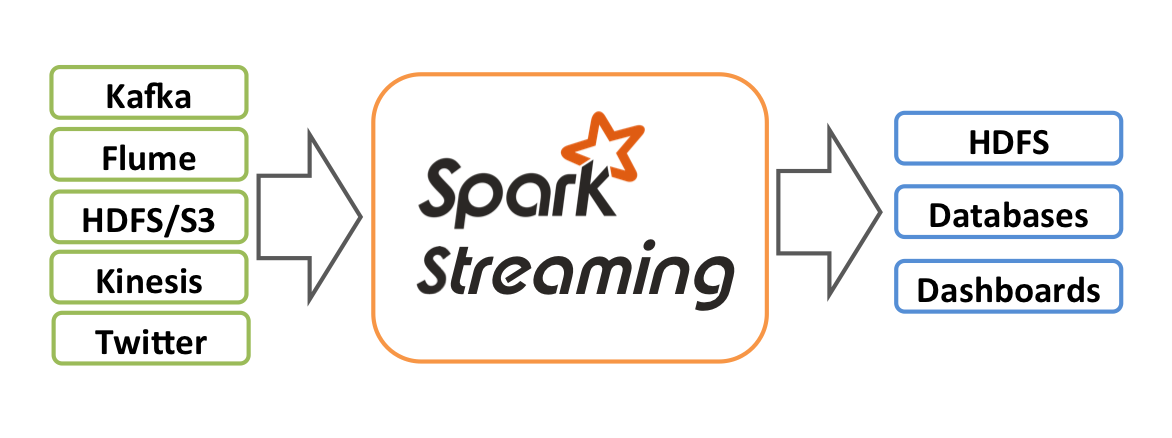
\includegraphics[width=0.75\textwidth]{pics/streaming-arch.png}\\
		\tiny\url{https://spark.apache.org/docs/3.3.1/streaming-programming-guide.html\#overview}
	}
	\uncover<2->{
		\centering
		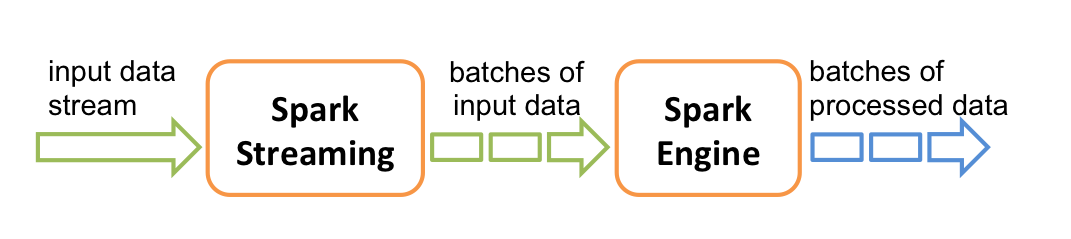
\includegraphics[width=0.75\textwidth]{pics/streaming-flow.png}\\
		\tiny\url{https://spark.apache.org/docs/3.3.1/streaming-programming-guide.html\#overview}
	}

\end{frame}

\section{Take-Away}
\begin{frame}{Take-Away}
	\begin{columns}
		\begin{column}{0.75\textwidth}
			\begin{itemize}
				\item Spark basiert auf der Idee von schreibgeschützten, verteilten Datensätzen
				\item RDDs können mit diversen Transformationen und Aktionen verarbeitet werden
				\item Aufwändige Transformationen können durch Lazy-Evaluation optimiert werden
				\item Fehlertoleranz wird durch simples Neuberechnen erzeugt
				\item Zusätzliche APIs für weitere Anwendungsfälle
			\end{itemize}
		\end{column}
		\begin{column}{0.25\textwidth}
			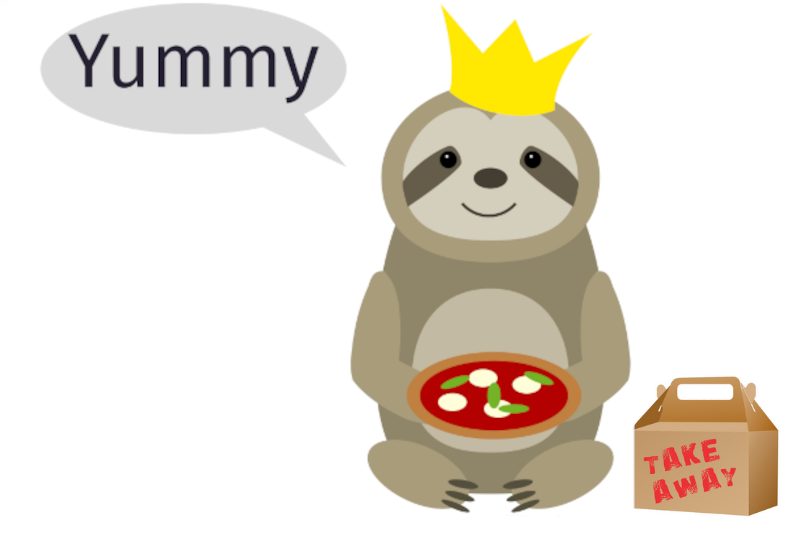
\includegraphics[width=\textwidth]{pics/sloth.png}\\
		\end{column}
	\end{columns}
\end{frame}

\section{Referenzen}
\begin{frame}[allowframebreaks]{Literatur}{Moodle}
	\printbibliography[keyword={moodle}]
\end{frame}

\begin{frame}[allowframebreaks]{Literatur}{Weiterführend}
	\printbibliography[notkeyword={moodle}]
\end{frame}

\end{document}